\section{Theoretical Analysis}

For this part, we used the scheme in Fig. \ref{fig:joaoscheme}, which takes into account the approximation of the OP-AMP as shown in Fig. \ref{fig:approximation}.

\begin{figure}[H]
    \centering
    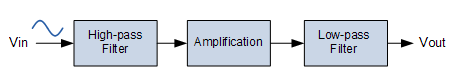
\includegraphics{esquemabunituh.PNG}
    \caption{Scheme used for Octave.}
    \label{fig:joaoscheme}
\end{figure}

\begin{figure}[H]
    \centering
    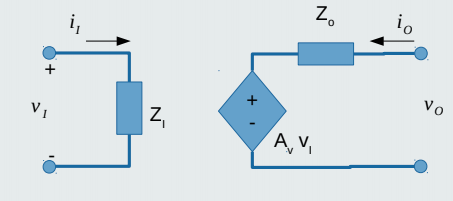
\includegraphics{slidespic.png}
    \caption{OP-AMP approximation, shown in theoretical classes (Source: Teacher's slides).}
    \label{fig:approximation}
\end{figure}

The results for this part are summarized in Tab. \ref{tab:valuesoctave}. As a sidenote, the cutoff frequencies are $f_{low} = 413.830Hz$ and $f_{high} = 2682.70Hz$.

\begin{table}[H]
    \centering
    \begin{tabular}{|c|c|}
    	\hline
        Variable & Unit [Hz, dB, -, -]\\ 
        \hline
        Central Frequency & 1053.65\\
        \hline
        Gaindb & 40.1602\\
        \hline
        Merit & 8.53488e-6\\
        \hline
        Clean Merit & 3.29139e-5\\
        \hline
    \end{tabular}
    \caption{Values obtained using the scheme in Fig. \ref{fig:joaoscheme}, implemented in Octave.}
    \label{tab:valuesoctave}
\end{table}

The input and output impedances are shown below in Tab. \ref{tab:octinput} and Tab. \ref{tab:octouput}, respectively. You can also check the frequency response in Fig. \ref{fig:octavefreq}.

\begin{table}[H]
    \centering
    \begin{tabular}{|c|c|}
    	\hline
        Impedance &  [VA]\\ 
        \hline
        $Z_{in}$ & 1000.00 + i(-686.595)\\ \hline
        $|Z_{in}|$ & 1213.02\\ \hline
    \end{tabular}
    \caption{Input impedance.}
    \label{tab:octinput}
\end{table}

\begin{table}[H]
    \centering
    \begin{tabular}{|c|c|}
    	\hline
        Impedance &  [VA]\\ 
        \hline
        $Z_{out}$ & 669.582 + i(-110.422)\\ \hline
        $|Z_{out}|$ & 818.280\\ \hline
    \end{tabular}
    \caption{Output impedance.}
    \label{tab:octoutput}
\end{table}

\begin{figure}[H]
    \centering
    \includegraphics[width = \linewidth]{../mat/gain_banda.png}
    \caption{Frequency response of the circuit shown in Fig. \ref{fig:joaoscheme}, in dB.}
    \label{fig:octavefreq}
\end{figure}